% Lista04_Q1.tex
% !TeX root = L04_RelFinal.tex
\section*{Lista de Exercícios 4}
\addcontentsline{toc}{chapter}{Lista de Exercícios 4}

\noindent \textbf{Data:} 07/10/2026

\section*{Resolução}
\subsection*{Questão 1}

\subsubsection*{Modelagem: Hipóteses}

\begin{enumerate}
  \item Regime permanente e transporte unidimensional na direção $x$.
  \item Propriedades constantes ($\rho$, $\Gamma^{\varphi}$) e velocidade $u$
        uniforme e positiva (escoamento de oeste para leste).
  \item Ausência de termo fonte.
  \item $\varphi$ prescrito nas duas fronteiras: $\varphi(0)=0$ e
        $\varphi(L)=1$.
\end{enumerate}

\subsubsection*{Equação governante e condições de contorno}

\begin{equation}
  \frac{\partial}{\partial x}\left(\rho\,u\,\varphi\right)
  =\frac{\partial}{\partial x}\!\left(\Gamma^{\varphi}\,
  \frac{\partial \varphi}{\partial x}\right),
  \qquad
  \varphi(0)=\varphi_0=0,\qquad \varphi(L)=\varphi_L=1 .
  \label{eq:advdif}
\end{equation}

O lado esquerdo representa o transporte advectivo de $\varphi$ e o lado
direito o transporte difusivo.

\subsubsection*{Parâmetros}

\[
\begin{array}{lll}
  \rho=1\ \mathrm{kg/m^{3}} & \Gamma^{\varphi}=1\ \mathrm{kg/(m\,s)} & L=1\ \mathrm{m}\\[2pt]
  \varphi_0=0 & \varphi_L=1 & u=0;\ 10;\ 50;\ 100\ \mathrm{m/s}
\end{array}
\]

\subsubsection*{Solução analítica}

Com $\rho u$ e $\Gamma^{\varphi}$ constantes, a Eq.~\eqref{eq:advdif} reduz-se a
$\varphi''-(\mathrm{Pe}_L/L)\,\varphi'=0$, cuja solução, aplicadas as condições
de contorno, é
\begin{equation}
  \varphi(x)=\frac{e^{\,\mathrm{Pe}_L\,x/L}-1}{e^{\,\mathrm{Pe}_L}-1},
  \qquad
  \mathrm{Pe}_L=\frac{\rho\,u\,L}{\Gamma^{\varphi}} ,
  \label{eq:analitica}
\end{equation}

À medida que $\mathrm{Pe}_L$ cresce, $\varphi$ permanece praticamente igual ao
valor de entrada ($\varphi_0=0$) em quase todo o domínio e a variação
concentra-se em uma camada limite junto a $x=L$, de espessura da ordem de
$\Gamma^{\varphi}/\rho u$.

\subsubsection*{Discretização por volumes finitos}

\subsubsection*{Malha}

O domínio $0\le x\le L$ é dividido em $N$ volumes de largura $\Delta x=L/N$,
com o nó no centro de cada volume (\emph{cell-centered}), de modo que
$x_m=(m-\tfrac12)\Delta x$. Mantém-se a notação $W$, $P$, $E$ para os nós e
$w$, $e$ para as faces. Nos volumes de fronteira a distância do nó ao contorno
é $\Delta x/2$.

\subsubsection*{Integração}

Integrando a Eq.~\eqref{eq:advdif} entre as faces $w$ e $e$ do volume $P$:
\begin{equation}
  F\,\varphi_e-F\,\varphi_w
  =\Gamma^{\varphi}\left.\frac{\partial\varphi}{\partial x}\right|_e
  -\Gamma^{\varphi}\left.\frac{\partial\varphi}{\partial x}\right|_w ,
  \qquad
  F=\rho\,u,\qquad D=\frac{\Gamma^{\varphi}}{\Delta x} .
  \label{eq:balanco}
\end{equation}

A Eq.~\eqref{eq:balanco} é exata; a aproximação está na função de interpolação
usada para avaliar $\varphi$ e $\partial\varphi/\partial x$ nas faces a partir
dos valores nodais. Em todos os casos chega-se à forma
\begin{equation}
  \boxed{\;A_P\,\varphi_P=A_W\,\varphi_W+A_E\,\varphi_E+B\;}
  \label{eq:geral}
\end{equation}
resolvida pelo TDMA. O parâmetro que governa o comportamento dos esquemas é o
número de Péclet de malha,
\[
  \mathrm{Pe}_{\Delta}=\frac{F}{D}=\frac{\rho\,u\,\Delta x}{\Gamma^{\varphi}} .
\]

\begin{table}[H]
\centering
\caption{Número de Péclet de malha para $N=20$ ($\Delta x=0{,}05$~m).}
\begin{tabular}{crrr}
\hline
$u$ (m/s) & $F$ & $D$ & $\mathrm{Pe}_{\Delta}$\\
\hline
0   & 0   & 20 & 0\\
10  & 10  & 20 & 0,5\\
50  & 50  & 20 & 2,5\\
100 & 100 & 20 & 5,0\\
\hline
\end{tabular}
\end{table}

\vspace{0.5cm}

%======================================================================
\subsubsection*{a) CDS para os termos advectivo e difusivo}

\subsubsection*{Função de interpolação}

No esquema de diferenças centrais admite-se variação linear de $\varphi$ entre
nós vizinhos:
\[
  \varphi_e=\frac{\varphi_P+\varphi_E}{2},\qquad
  \varphi_w=\frac{\varphi_W+\varphi_P}{2},
\]
\[
  \left.\frac{\partial\varphi}{\partial x}\right|_e=\frac{\varphi_E-\varphi_P}{\Delta x},\qquad
  \left.\frac{\partial\varphi}{\partial x}\right|_w=\frac{\varphi_P-\varphi_W}{\Delta x}.
\]

\subsubsection*{Volumes internos ($2\le m\le N-1$)}

Substituindo na Eq.~\eqref{eq:balanco} e agrupando:
\[
  A_E=D-\frac{F}{2},\qquad
  A_W=D+\frac{F}{2},\qquad
  A_P=2D,\qquad
  B=0 .
\]

\subsubsection*{Volume de fronteira 1 ($\varphi_0$ prescrito)}

A face oeste coincide com o contorno: $\varphi_w=\varphi_0$ e o gradiente é
avaliado em meia largura de volume,
$\left.\partial\varphi/\partial x\right|_w=(\varphi_P-\varphi_0)/(\Delta x/2)$:
\[
  A_E=D-\frac{F}{2},\qquad
  A_W=0,\qquad
  A_P=3D+\frac{F}{2},\qquad
  B_1=\left(2D+F\right)\varphi_0=0 .
\]

\subsubsection*{Volume de fronteira $N$ ($\varphi_L$ prescrito)}

Analogamente, $\varphi_e = 1$ e
$\left.\partial\varphi/\partial x\right|_e=(\varphi_L-\varphi_P)/(\Delta x/2)$:
\[
  A_E=0,\qquad
  A_W=D+\frac{F}{2},\qquad
  A_P=3D-\frac{F}{2},\qquad
  B_N=\left(2D-F\right)
\]

\subsubsection*{Resultados}

\begin{figure}[H]
\centering
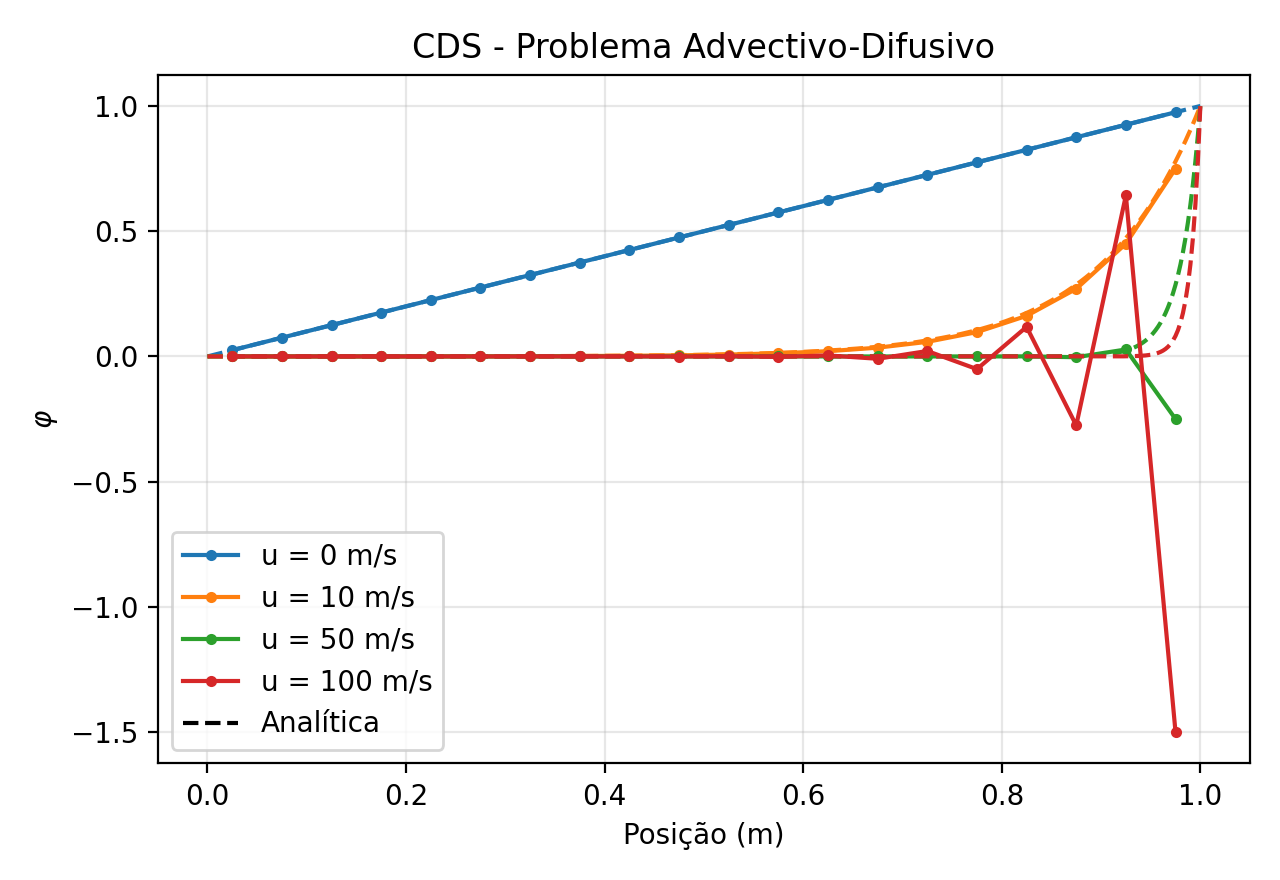
\includegraphics[width=0.75\textwidth]{L04_Q1_CDS.png}
\caption{CDS, $N=20$. Linhas cheias: solução numérica; tracejadas: solução
analítica.}
\end{figure}

\begin{table}[H]
\centering
\caption{CDS, $N=20$. O erro é o desvio máximo nodal em relação à
Eq.~\eqref{eq:analitica}.}
\begin{tabular}{crrrr}
\hline
$u$ (m/s) & $\mathrm{Pe}_{\Delta}$ & $A_E$ & $|e|_{\max}$ & $\varphi_{\min}$\\
\hline
0   & 0   & 20      & 0,0000 & 0,0250\\
10  & 0,5 & 15      & 0,0288 & 0,0000\\
50  & 2,5 & $-5$    & 0,5365 & $-0{,}2500$\\
100 & 5,0 & $-30$   & 1,5821 & $-1{,}5000$\\
\hline
\end{tabular}
\end{table}

Para $u=0$ a solução é linear e o CDS a reproduz exatamente. Para $u=10$~m/s
($\mathrm{Pe}_{\Delta}=0{,}5$) o resultado acompanha a solução analítica, com
erro máximo de $0{,}029$. Para $u=50$ e $100$~m/s, porém, a solução apresenta
oscilações espaciais sem significado físico, com valores negativos e fora do
intervalo $[0,1]$ imposto pelas fronteiras.

A razão está no coeficiente $A_E=D-F/2$, que se torna negativo quando
\[
  \mathrm{Pe}_{\Delta}=\frac{F}{D}>2 .
\]
Isso ocorre porque o CDS calcula $\varphi$ na face como a média dos dois nós vizinhos, sem considerar o sentido do escoamento. Quando a advecção domina ($\mathrm{Pe}_{\Delta}>2$), essa média dá peso demais ao nó leste, e a solução passa a oscilar.

\vspace{0.5cm}

%======================================================================
\subsubsection*{b) UDS para o termo advectivo e CDS para o difusivo}

\subsubsection*{Função de interpolação}

No esquema \emph{upwind} o valor de $\varphi$ na face é o do nó a oeste.
Como $u>0$:
\[
  \varphi_e=\varphi_P,\qquad \varphi_w=\varphi_W ,
\]
mantendo-se as diferenças centrais para os gradientes do termo difusivo.

\subsubsection*{Volumes internos ($2\le m\le N-1$)}
\[
  A_E=D,\qquad
  A_W=D+F,\qquad
  A_P=2D+F,\qquad
  B=0 .
\]

\subsubsection*{Volume de fronteira 1 ($\varphi_0$ prescrito)}

O valor a montante da face oeste é o próprio contorno, $\varphi_w=\varphi_0$:
\[
  A_E=D,\qquad
  A_W=0,\qquad
  A_P=3D+F,\qquad
  B_1=\left(2D+F\right)\varphi_0=0 .
\]

\subsubsection*{Volume de fronteira $N$ ($\varphi_L$ prescrito)}

Na extremidade direita, o valor à leste é o do nó, $\varphi_e=\varphi_P$, de modo que
o contorno ($\varphi_L = 1$) aparece apenas no termo difusivo:
\[
  A_E=0,\qquad
  A_W=D+F,\qquad
  A_P=3D+F,\qquad
  B_N=2D\,\varphi_L .
\]

\subsubsection*{Resultados}

\begin{figure}[H]
\centering
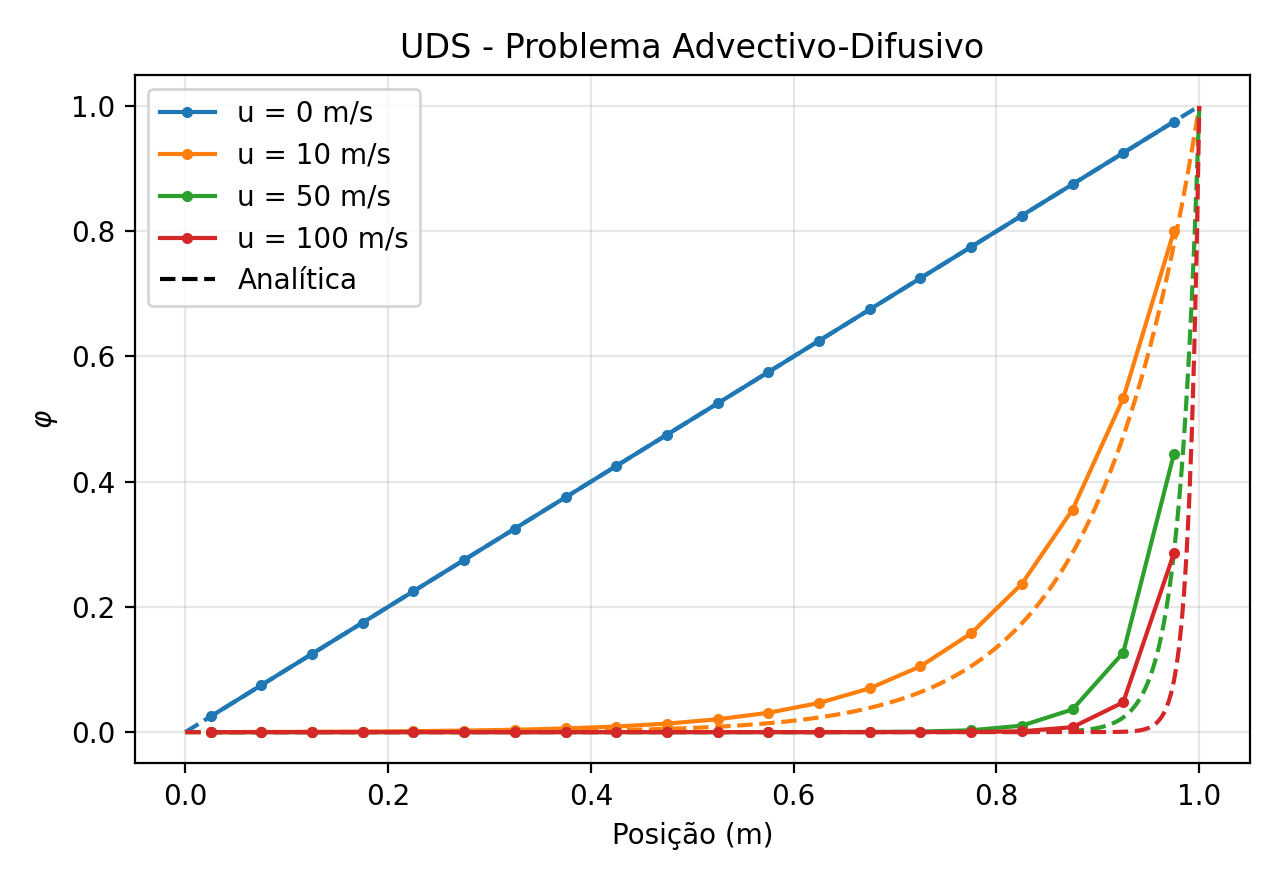
\includegraphics[width=0.75\textwidth]{L04_Q1_UDS.png}
\caption{UDS, $N=20$. Linhas cheias: solução numérica; tracejadas: solução
analítica.}
\end{figure}

\begin{table}[H]
\centering
\caption{UDS, $N=20$.}
\begin{tabular}{crrrr}
\hline
$u$ (m/s) & $\mathrm{Pe}_{\Delta}$ & $A_E$ & $|e|_{\max}$ & $\varphi_{\min}$\\
\hline
0   & 0   & 20 & 0,0000 & 0,0250\\
10  & 0,5 & 20 & 0,0689 & 0,0001\\
50  & 2,5 & 20 & 0,1579 & 0,0000\\
100 & 5,0 & 20 & 0,2036 & 0,0000\\
\hline
\end{tabular}
\end{table}

Todos os coeficientes são positivos para qualquer $\mathrm{Pe}_{\Delta}$, de modo que a solução converge sem oscilações.

O custo é a perda de exatidão. O UDS é um esquema de primeira ordem: seu erro é proporcional ao tamanho da malha, $\Delta x$, enquanto no CDS é proporcional a $\Delta x^{2}$. Mesmo para $u=10$~m/s, em que o CDS é estável, o UDS é menos exato ($0{,}069$ contra $0{,}029$).

\vspace{0.5cm}

%======================================================================
\subsubsection*{c) WUDS para os termos advectivo e difusivo}

\subsubsection*{Função de interpolação}

O WUDS pondera as aproximações central e \emph{upwind} por meio de dois
coeficientes que dependem do Péclet de malha:
\[
  \varphi_e=\left(\tfrac12+\alpha\right)\varphi_P
           +\left(\tfrac12-\alpha\right)\varphi_E ,
  \qquad
  \left.\Gamma^{\varphi}\frac{\partial\varphi}{\partial x}\right|_e
  =\beta\,D\left(\varphi_E-\varphi_P\right),
\]
\[
  \varphi_w=\left(\tfrac12+\alpha\right)\varphi_W
           +\left(\tfrac12-\alpha\right)\varphi_P ,
  \qquad
  \left.\Gamma^{\varphi}\frac{\partial\varphi}{\partial x}\right|_w
  =\beta\,D\left(\varphi_P-\varphi_W\right),
\]
, com
\begin{equation}
  \alpha=\frac{\mathrm{Pe}_{\Delta}^{2}}{10+2\,\mathrm{Pe}_{\Delta}^{2}},
  \qquad
  \beta=\frac{1+0{,}005\,\mathrm{Pe}_{\Delta}^{2}}{1+0{,}05\,\mathrm{Pe}_{\Delta}^{2}} .
\end{equation}

Os limites recuperam os esquemas anteriores: para $\mathrm{Pe}_{\Delta}\to0$,
$\alpha\to0$ e $\beta\to1$ (CDS); para $\mathrm{Pe}_{\Delta}\to\infty$,
$\alpha\to\tfrac12$ (UDS) e $\beta\to0{,}1$, reduzindo a difusão onde a
advecção domina. Como a malha é uniforme e as propriedades constantes,
$\alpha$ e $\beta$ são iguais em todas as faces internas.

\subsubsection*{Volumes internos ($2\le m\le N-1$)}
\[
\begin{aligned}
  A_E&=\beta D-F\left(\tfrac12-\alpha\right), &
  A_W&=\beta D+F\left(\tfrac12+\alpha\right), \\[4pt]
  A_P&=2\left(\beta D+\alpha F\right), &
  B&=0 .
\end{aligned}
\]

\subsubsection*{Volumes de fronteira}

Nas faces de contorno a distância entre o nó e a fronteira é $\dfrac{\Delta x}{2}$;
os coeficientes são então avaliados com o Péclet correspondente,
\[
  \mathrm{Pe}_{b}=\frac{\rho\,u\,(\Delta x/2)}{\Gamma^{\varphi}},
  \qquad
  \alpha_b=\alpha(\mathrm{Pe}_b),\qquad \beta_b=\beta(\mathrm{Pe}_b),
\]
e a condutância difusiva ($ \Gamma^\varphi$) passa a $2\beta_b D$.

\emph{Volume 1} -- face oeste no contorno, com $\varphi_w=\varphi_0$:
\[
\begin{aligned}
  A_E&=\beta D-F\left(\tfrac12-\alpha\right), &
  A_W&=0, \\[4pt]
  A_P&=F\left(\tfrac12+\alpha\right)+\beta D+2\beta_b D, &
  B_1&=\left(F+2\beta_b D\right)\varphi_0=0 .
\end{aligned}
\]

\emph{Volume $N$} -- face leste no contorno, com
$\varphi_e=\left(\tfrac12+\alpha_b\right)\varphi_P
+\left(\tfrac12-\alpha_b\right)\varphi_L$:
\[
\begin{aligned}
  A_E&=0, &
  A_W&=\beta D+F\left(\tfrac12+\alpha\right), \\[4pt]
  A_P&=F\left(\alpha+\alpha_b\right)+\beta D+2\beta_b D, &
  B_N&=\left[\,2\beta_b D-F\left(\tfrac12-\alpha_b\right)\right]\varphi_L .
\end{aligned}
\]

\subsubsection*{i) Malha com 20 volumes, $u=0$; 10; 50 e 100 m/s}

\begin{figure}[H]
\centering
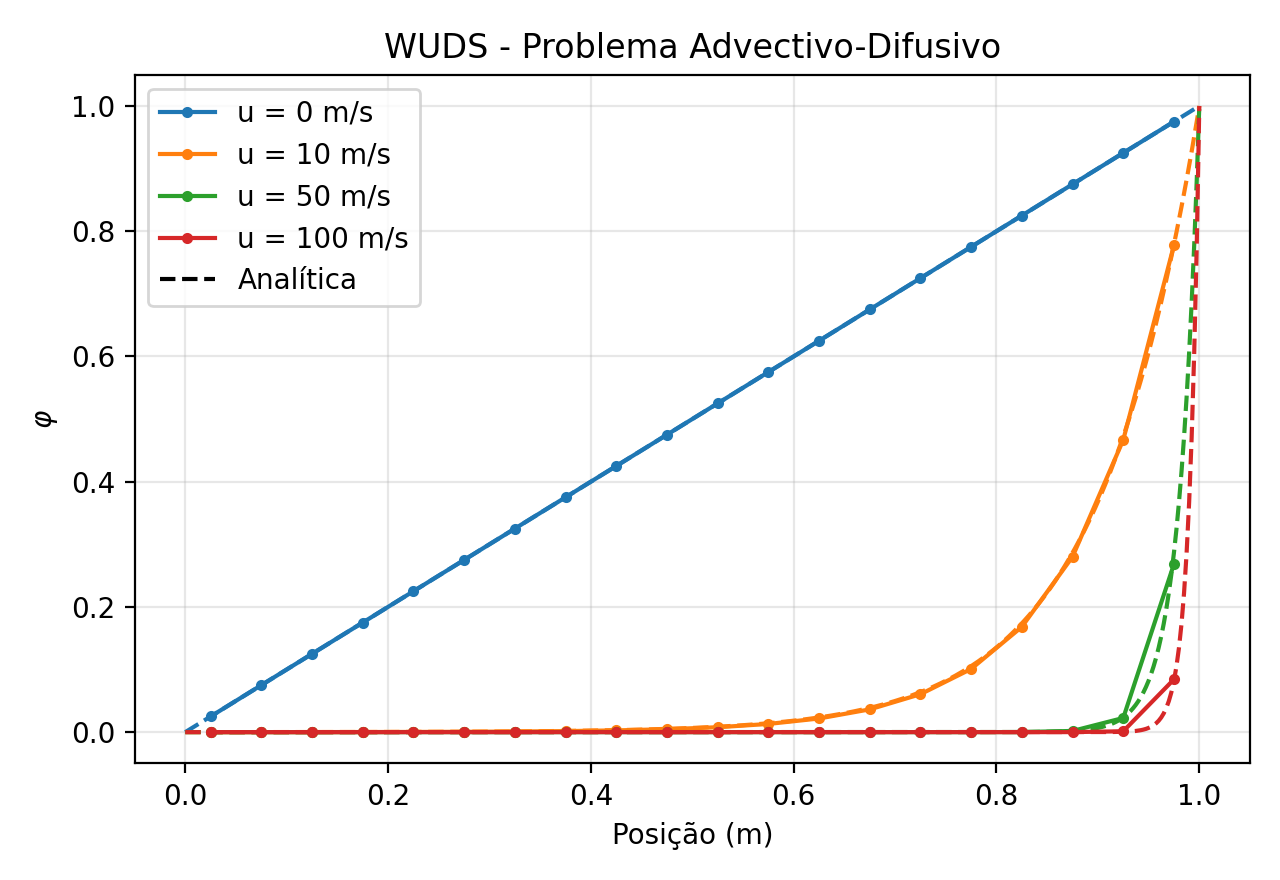
\includegraphics[width=0.75\textwidth]{L04_Q1_WUDS.png}
\caption{WUDS, $N=20$. Linhas cheias: solução numérica; tracejadas: solução
analítica.}
\end{figure}

\begin{table}[H]
\centering
\caption{WUDS, $N=20$.}
\begin{tabular}{crrrrrr}
\hline
$u$ (m/s) & $\mathrm{Pe}_{\Delta}$ & $\alpha$ & $\beta$ & $A_E$ & $|e|_{\max}$ & $\varphi_{\min}$\\
\hline
0   & 0   & 0,0000 & 1,0000 & 20,00 & 0,0000 & 0,0250\\
10  & 0,5 & 0,0238 & 0,9889 & 15,02 & 0,0064 & 0,0000\\
50  & 2,5 & 0,2778 & 0,7857 & 4,60  & 0,0181 & 0,0000\\
100 & 5,0 & 0,4167 & 0,5000 & 1,67  & 0,0022 & 0,0000\\
\hline
\end{tabular}
\end{table}

O WUDS reúne as qualidades dos dois esquemas anteriores. O coeficiente $A_E$
permanece positivo em todas as velocidades, de modo que a solução converge sem oscilações, como no UDS; ao mesmo tempo, as curvas numéricas praticamente
coincidem com as analíticas, com erro máximo de $0{,}018$, uma ordem de
grandeza abaixo do UDS. Isso ocorre porque $\alpha$ e $\beta$ são ajustes da
solução exata do problema unidimensional sem fonte: a interpolação entre nós
aproxima o próprio perfil exponencial da Eq.~\eqref{eq:analitica}, e não uma
reta (CDS) ou um degrau (UDS).

\subsubsection*{ii) $u=60$ m/s, malhas com 10, 20, 50 e 100 volumes}

\begin{figure}[H]
\centering
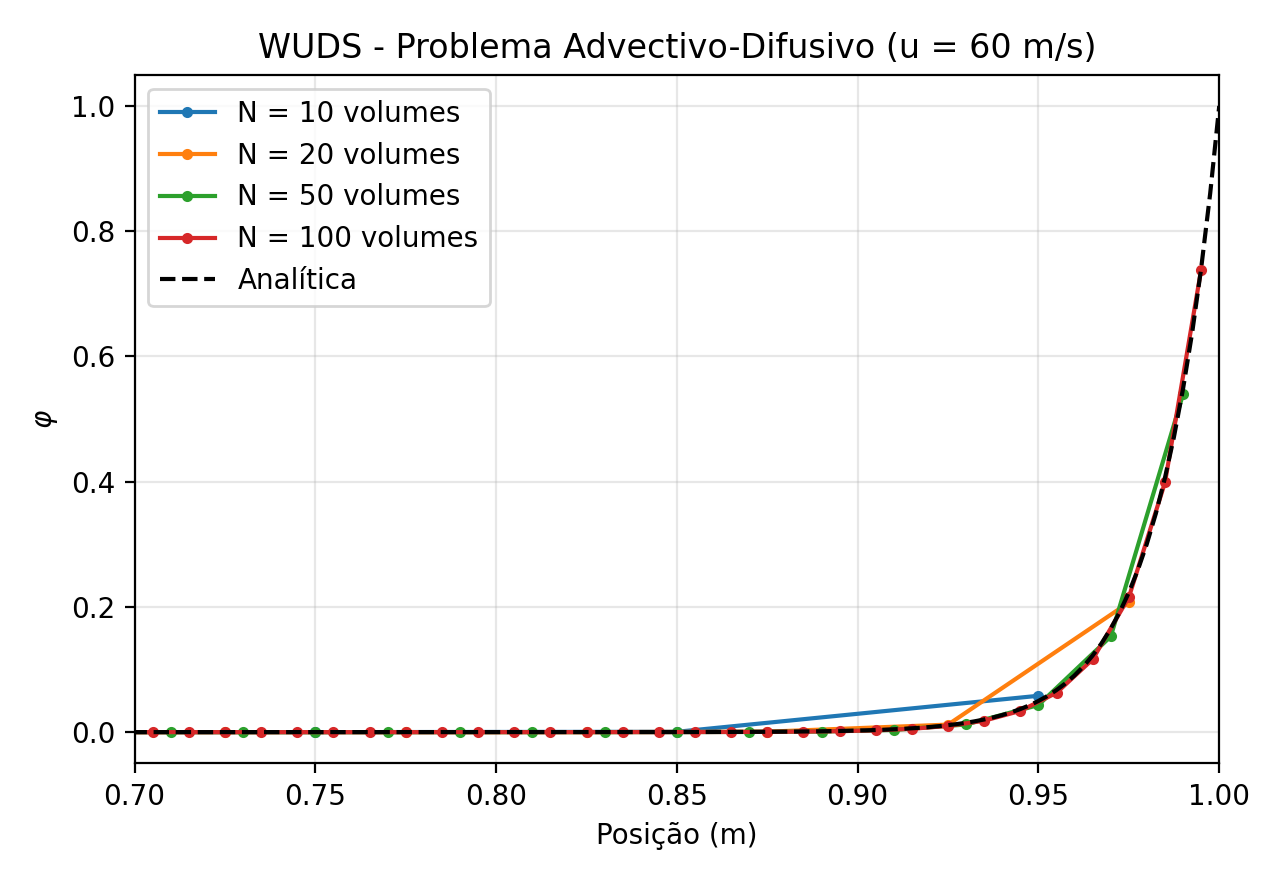
\includegraphics[width=0.75\textwidth]{L04_Q1_WUDS_malhas.png}
\caption{WUDS, $u=60$~m/s ($\mathrm{Pe}_L=60$): detalhe da região
$0{,}7\le x\le1$, onde se concentra a variação de $\varphi$.}
\end{figure}

\begin{table}[H]
\centering
\caption{WUDS, $u=60$~m/s: influência do refino da malha.}
\begin{tabular}{crrrrr}
\hline
$N$ & $\Delta x$ (m) & $\mathrm{Pe}_{\Delta}$ & $\alpha$ & $\beta$ & $|e|_{\max}$\\
\hline
10  & 0,100 & 6,0 & 0,4390 & 0,4214 & 0,0083\\
20  & 0,050 & 3,0 & 0,3214 & 0,7207 & 0,0161\\
50  & 0,020 & 1,2 & 0,1118 & 0,9396 & 0,0125\\
100 & 0,010 & 0,6 & 0,0336 & 0,9841 & 0,0077\\
\hline
\end{tabular}
\end{table}

As quatro malhas fornecem soluções estáveis, sem oscilações, e com valores
nodais próximos da solução analítica -- inclusive a malha de 10 volumes, com
$\mathrm{Pe}_{\Delta}=6$, condição em que o CDS seria inviável. Com o refino,
$\mathrm{Pe}_{\Delta}$ diminui, $\alpha\to0$ e $\beta\to1$: o esquema
aproxima-se gradualmente do CDS.

O erro máximo nodal não decresce continuamente com $N$. A camada limite tem
espessura da ordem de $\Gamma^{\varphi}/\rho u\approx0{,}017$~m, menor que o
próprio volume da malha mais grosseira. Com $N=10$ há um único nó próximo dessa
região (em $x=0{,}95$~m), onde $\varphi$ ainda é pequeno, e todos os demais
estão no trecho em que $\varphi\approx0$; o erro nodal é baixo, mas o perfil
dentro da camada limite simplesmente não é representado. Ao refinar, os nós
passam a ocupar a região de gradiente elevado, onde os desvios são
naturalmente maiores, e somente a partir daí o erro passa a cair com
$\Delta x$ ($0{,}0161\to0{,}0125\to0{,}0077$). O ganho real do refino é,
portanto, a \emph{resolução} da camada limite, bem descrita apenas com 50 e
100 volumes.

\vspace{0.5cm}

%======================================================================
\subsubsection*{Comparação dos esquemas com a solução analítica}

\begin{table}[H]
\centering
\caption{Erro máximo nodal em relação à solução analítica ($N=20$).}
\begin{tabular}{crrrr}
\hline
$u$ (m/s) & $\mathrm{Pe}_{\Delta}$ & CDS & UDS & WUDS\\
\hline
0   & 0   & 0,0000 & 0,0000 & 0,0000\\
10  & 0,5 & 0,0288 & 0,0689 & 0,0064\\
50  & 2,5 & 0,5365 & 0,1579 & 0,0181\\
100 & 5,0 & 1,5821 & 0,2036 & 0,0022\\
\hline
\end{tabular}
\end{table}

Portanto, pode-se concluir que, em problemas advectivos dominantes, o esquema de interpolação deve levar em conta a direção do escoamento. O CDS ignora essa informação e falha para $\mathrm{Pe}_{\Delta}>2$; o UDS a considera integralmente, ao custo do erro diretamente proporcional ao tamanho de malha $\Delta x$ e não ao quadrado do tamanho de malha $\Delta x^2$, como no CDS; o WUDS pondera as duas contribuições conforme o Péclet local e reproduz a solução analítica com boa exatidão mesmo em malhas grosseiras.

% Lista04_Q2.tex
% !TeX root = L04_RelFinal.tex
% Requer no preâmbulo do arquivo raiz: \usepackage{amsmath}, \usepackage{graphicx}, \usepackage{float}
\subsection*{Questão 2}

\subsubsection*{Modelagem: Hipóteses}

\begin{enumerate}
  \item Regime permanente e transporte bidimensional no plano $xy$.
  \item Propriedades constantes ($\rho$, $k$, $c_p$).
  \item Campo de velocidades conhecido e uniforme, $\mathbf{V}=(u,v)$, com
        componentes de qualquer sinal (a figura do enunciado ilustra o caso
        $u>0$, $v>0$).
  \item Sem geração interna de calor; o termo fonte de troca pelas faces da
        placa é introduzido apenas na última parte.
\end{enumerate}

\subsubsection*{Equação governante e condições de contorno}

O balanço de energia em um elemento $dx\,dy$ soma as contribuições das quatro
faces. Dividindo a equação da energia por $c_p$ (constante):
\begin{equation}
  \frac{\partial}{\partial x}\left(\rho\,u\,T\right)
  +\frac{\partial}{\partial y}\left(\rho\,v\,T\right)
  =\frac{\partial}{\partial x}\left(\Gamma\,\frac{\partial T}{\partial x}\right)
  +\frac{\partial}{\partial y}\left(\Gamma\,\frac{\partial T}{\partial y}\right),
  \qquad \Gamma=\frac{k}{c_p},
  \label{eq:q2gov}
\end{equation}
\[
  T(x,0)=\operatorname{sen}\left(\frac{\pi x}{a}\right),\qquad
  T(x,b)=0,\qquad T(0,y)=0,\qquad T(a,y)=0 .
\]

\subsubsection*{Adimensionalização}

Com $x^*=x/a$ e $y^*=y/b$, o domínio passa a ser sempre o quadrado unitário.
Usando $\partial/\partial x=(1/a)\,\partial/\partial x^*$ e
$\partial/\partial y=(1/b)\,\partial/\partial y^*$, e multiplicando a
Eq.~\eqref{eq:q2gov} por $a^2/\Gamma$:
\begin{equation}
  \mathrm{Pe}_a\,\frac{\partial T}{\partial x^*}
  +\mathrm{Pe}_b\left(\frac{a}{b}\right)^{2}\frac{\partial T}{\partial y^*}
  =\frac{\partial^2T}{\partial x^{*2}}
  +\left(\frac{a}{b}\right)^{2}\frac{\partial^2T}{\partial y^{*2}},
  \qquad
  \mathrm{Pe}_a=\frac{\rho\,u\,a}{\Gamma},\quad
  \mathrm{Pe}_b=\frac{\rho\,v\,b}{\Gamma},
  \label{eq:q2adim}
\end{equation}
\[
  T(x^*,0)=\operatorname{sen}(\pi x^*),\qquad
  T(x^*,1)=T(0,y^*)=T(1,y^*)=0 .
\]

O problema fica governado por três grupos adimensionais: $\mathrm{Pe}_a$,
$\mathrm{Pe}_b$ e a razão de aspecto $b/a$. Em uma malha de
$N_x\times N_y$ volumes, os números de Péclet de malha se relacionam com eles
por
\[
  \mathrm{Pe}_{\Delta x}=\frac{\rho\,u\,\Delta x}{\Gamma}=\frac{\mathrm{Pe}_a}{N_x},
  \qquad
  \mathrm{Pe}_{\Delta y}=\frac{\rho\,v\,\Delta y}{\Gamma}=\frac{\mathrm{Pe}_b}{N_y}.
\]
Nas simulações adotou-se $\rho=\Gamma=a=1$, de modo que $u$ coincide
numericamente com $\mathrm{Pe}_a$.

\subsubsection*{Discretização por volumes finitos}

\subsubsection*{Malha e integração}

O domínio é dividido em $N_x\times N_y$ volumes retangulares de dimensões
$\Delta x=a/N_x$ e $\Delta y=b/N_y$, com nós no centro dos volumes. Integrando
a Eq.~\eqref{eq:q2gov} no volume $P$ (profundidade unitária), cada fluxo é
multiplicado pelo comprimento da face que atravessa:
\[
  F_eT_e-F_wT_w+F_nT_n-F_sT_s
  =\left.\Gamma\frac{\partial T}{\partial x}\right|_e\!\Delta y
  -\left.\Gamma\frac{\partial T}{\partial x}\right|_w\!\Delta y
  +\left.\Gamma\frac{\partial T}{\partial y}\right|_n\!\Delta x
  -\left.\Gamma\frac{\partial T}{\partial y}\right|_s\!\Delta x ,
\]
\[
  F_e=F_w=\rho\,u\,\Delta y,\qquad
  F_n=F_s=\rho\,v\,\Delta x,\qquad
  D_e=\frac{\Gamma\,\Delta y}{\Delta x},\qquad
  D_n=\frac{\Gamma\,\Delta x}{\Delta y}.
\]
Com essas definições, $F_e/D_e=\mathrm{Pe}_{\Delta x}$ e
$F_n/D_n=\mathrm{Pe}_{\Delta y}$.

\subsubsection*{Função de interpolação WUDS}

Em cada direção, o valor na face e o fluxo difusivo são ponderados pelos
coeficientes do WUDS, calculados com o Péclet de malha daquela direção:
\[
  T_e=\left(\tfrac12+\alpha_x\right)T_P+\left(\tfrac12-\alpha_x\right)T_E,
  \qquad
  \left.\Gamma\frac{\partial T}{\partial x}\right|_e\Delta y=\beta_x\,D_e\,(T_E-T_P),
\]
\[
  T_n=\left(\tfrac12+\alpha_y\right)T_P+\left(\tfrac12-\alpha_y\right)T_N,
  \qquad
  \left.\Gamma\frac{\partial T}{\partial y}\right|_n\Delta x=\beta_y\,D_n\,(T_N-T_P),
\]
e analogamente para as faces $w$ e $s$, com
\[
  \alpha=\operatorname{sinal}(\mathrm{Pe}_\Delta)\,
  \frac{\mathrm{Pe}_\Delta^{2}}{10+2\,\mathrm{Pe}_\Delta^{2}},\qquad
  \beta=\frac{1+0{,}005\,\mathrm{Pe}_\Delta^{2}}{1+0{,}05\,\mathrm{Pe}_\Delta^{2}} .
\]
O sinal de $\alpha$ acompanha o do Péclet de malha. Com $u>0$, o peso maior,
$\tfrac12+\alpha$, vai para $T_P$, que está a montante da face $e$; com
$u<0$, $\alpha<0$ e o peso maior passa para $T_E$, que se torna o nó de
montante. Assim as mesmas expressões valem para qualquer sentido do
escoamento.

\subsubsection*{Volumes internos}

Substituindo no balanço e agrupando:
\begin{equation}
  \boxed{\;A_P\,T_P=A_E\,T_E+A_W\,T_W+A_N\,T_N+A_S\,T_S+B\;}
\end{equation}
\[
\begin{aligned}
  A_E&=\beta_xD_e-F_e\left(\tfrac12-\alpha_x\right), &
  A_W&=\beta_xD_e+F_e\left(\tfrac12+\alpha_x\right),\\[4pt]
  A_N&=\beta_yD_n-F_n\left(\tfrac12-\alpha_y\right), &
  A_S&=\beta_yD_n+F_n\left(\tfrac12+\alpha_y\right),\\[4pt]
  A_P&=A_E+A_W+A_N+A_S, & B&=0 .
\end{aligned}
\]
A igualdade $A_P=\sum A_{nb}$ decorre da conservação da massa
($F_e=F_w$, $F_n=F_s$) e da ausência de termo fonte. Com $\alpha$ com sinal,
os coeficientes valem para $u$ e $v$ positivos ou negativos, e permanecem
positivos em toda a faixa de Péclet.

\subsubsection*{Volumes de fronteira}

Como as direções $x$ e $y$ são independentes, cada direção contribui
separadamente para $A_P$ e $B$; os volumes de canto recebem as duas
contribuições de contorno. Nas faces de contorno a distância entre o nó e a
fronteira é $\dfrac{\Delta x}{2}$, e $\alpha_b$, $\beta_b$ são avaliados com
${\mathrm{Pe}}_{\Delta x/2}$; a condutância difusiva passa a $2\beta_bD$.

Em todas as faces de contorno com temperatura prescrita adota-se a mesma
regra: o valor advectado pela face é interpolado pelo WUDS entre o contorno e
o nó, à meia distância. Na face sul, por exemplo,
\[
  T_s=\left(\tfrac12+\alpha_{yb}\right)T_b+\left(\tfrac12-\alpha_{yb}\right)T_P ,
\]
e, na face norte,
$T_n=\left(\tfrac12+\alpha_{yb}\right)T_P+\left(\tfrac12-\alpha_{yb}\right)T_b$.
Como $\alpha_{yb}$ tem o sinal de $v$, a interpolação favorece
automaticamente o lado de montante, seja ele o contorno (face de entrada) ou
o nó (face de saída), e o código não precisa saber por qual face o
escoamento entra.

Para a direção $y$ (a direção $x$ é análoga, trocando $n,s,y$ por $e,w,x$):

\emph{Volume interno em $y$:}
\begin{align*}
  A_S&=\beta_yD_n+F_n\left(\tfrac12+\alpha_y\right), &
  A_N&=\beta_yD_n-F_n\left(\tfrac12-\alpha_y\right),\\
  A_P^{(y)}&=A_N+A_S, & B^{(y)}&=0 .
\end{align*}

\emph{Fronteira sul:}
\begin{align*}
  A_S&=0, & A_P^{(y)}&=F_n\left(\alpha_y+\alpha_{yb}\right)+\beta_yD_n+2\beta_{yb}D_n,\\
  & & B^{(y)}&=\left[F_n\left(\tfrac12+\alpha_{yb}\right)+2\beta_{yb}D_n\right]T_b .
\end{align*}

\emph{Fronteira norte:}
\begin{align*}
  A_N&=0, & A_P^{(y)}&=F_n\left(\alpha_y+\alpha_{yb}\right)+\beta_yD_n+2\beta_{yb}D_n,\\
  & & B^{(y)}&=\left[2\beta_{yb}D_n-F_n\left(\tfrac12-\alpha_{yb}\right)\right]T_b .
\end{align*}

Os coeficientes finais são $A_P=A_P^{(x)}+A_P^{(y)}$ e $B=B^{(x)}+B^{(y)}$.

A interpolação é indispensável na face de saída. Usando diretamente $T_n=T_b$
no fluxo advectivo da face norte com $v>0$, a parcela de $A_P$ seria
$F_n(\alpha_y-\tfrac12)+\beta_yD_n+2\beta_{yb}D_n$, que fica menor que $A_S$
para $\mathrm{Pe}_{\Delta y}>2\beta_{yb}\approx2$: o nó junto à saída passaria
a valer mais que o vizinho a montante. No caso unidimensional de verificação
(Tabela~\ref{tab:q2_1Dv}) essa alternativa produziu erro de $2{,}26$ para
$\mathrm{Pe}_{\Delta y}=5$, contra $0{,}0022$ com a interpolação WUDS.

\subsubsection*{Verificação dos coeficientes}

Se todos os contornos estiverem na mesma temperatura, a solução tem de ser
uniforme e igual a ela. Isso exige, em todos os volumes,
\[
  A_P=A_E+A_W+A_N+A_S+\frac{B}{T_b},
\]
o que foi conferido numericamente: com os quatro contornos a $T=1$, malha
$10\times15$ e velocidades de ambos os sinais ($u=1$, $v=3$; $u=50$,
$v=150$; $u=-50$, $v=150$; $u=100$, $v=-30$; $u=v=-80$), a solução obtida
foi $T=1$ em todos os volumes, com desvio máximo de $10^{-11}$.

\subsubsection*{Solução do sistema: TDMA linha a linha}

Em 2D cada volume se liga a quatro vizinhos e a matriz deixa de ser
tridiagonal. O sistema é resolvido de forma iterativa, linha a linha: ao
resolver a linha horizontal $j$, os vizinhos norte e sul são tratados como
conhecidos (último valor disponível) e transferidos ao termo independente,
\[
  A_P\,T_P=A_E\,T_E+A_W\,T_W+\underbrace{A_N\,T_N+A_S\,T_S+B}_{d},
\]
de modo que cada linha é um problema tridiagonal resolvido pelo TDMA, com
$A_m=A_P$, $B_m=-A_E$, $C_m=-A_W$ e $D_m=d$. O procedimento é:

\begin{enumerate}
  \item Inicializar $T=0$ em todos os volumes;
  \item Calcular $A_P$, $A_E$, $A_W$, $A_N$, $A_S$ e $B$ uma única vez
        (problema linear);
  \item Para cada linha $j$, de sul para norte, montar $d$ com os valores
        atuais das linhas $j-1$ e $j+1$ e resolver a linha pelo TDMA,
        sobrescrevendo $T$;
  \item Avaliar $\max|T^{k+1}-T^{k}|$; se inferior a $\varepsilon$, encerrar;
        caso contrário, voltar ao passo~3.
\end{enumerate}

Adotou-se $\varepsilon=10^{-8}$ e, nos estudos de convergência de malha,
$\varepsilon=10^{-10}$, para que o erro de iteração ficasse muito abaixo do
erro de discretização.

\vspace{0.5cm}

%======================================================================
\subsubsection*{Caso limite 1: $u=v=0$ (condução pura)}

Sem escoamento, a Eq.~\eqref{eq:q2gov} reduz-se à equação de Laplace,
$\partial^2T/\partial x^2+\partial^2T/\partial y^2=0$. Por separação de
variáveis, com $T=\operatorname{sen}(\pi x/a)\,g(y)$, obtém-se
$g''-(\pi/a)^2g=0$, com $g(0)=1$ e $g(b)=0$, cuja solução fornece
\begin{equation}
  T(x,y)=\operatorname{sen}\left(\frac{\pi x}{a}\right)
  \frac{\operatorname{senh}\left[\pi(b-y)/a\right]}{\operatorname{senh}(\pi b/a)} .
  \label{eq:q2laplace}
\end{equation}

O perfil vertical não é linear, como seria em condução 1D: enquanto o calor
sobe a partir da base, parte dele escoa lateralmente para as paredes em
$T=0$, e a temperatura decai de forma aproximadamente exponencial com $y$.

\begin{figure}[H]
\centering
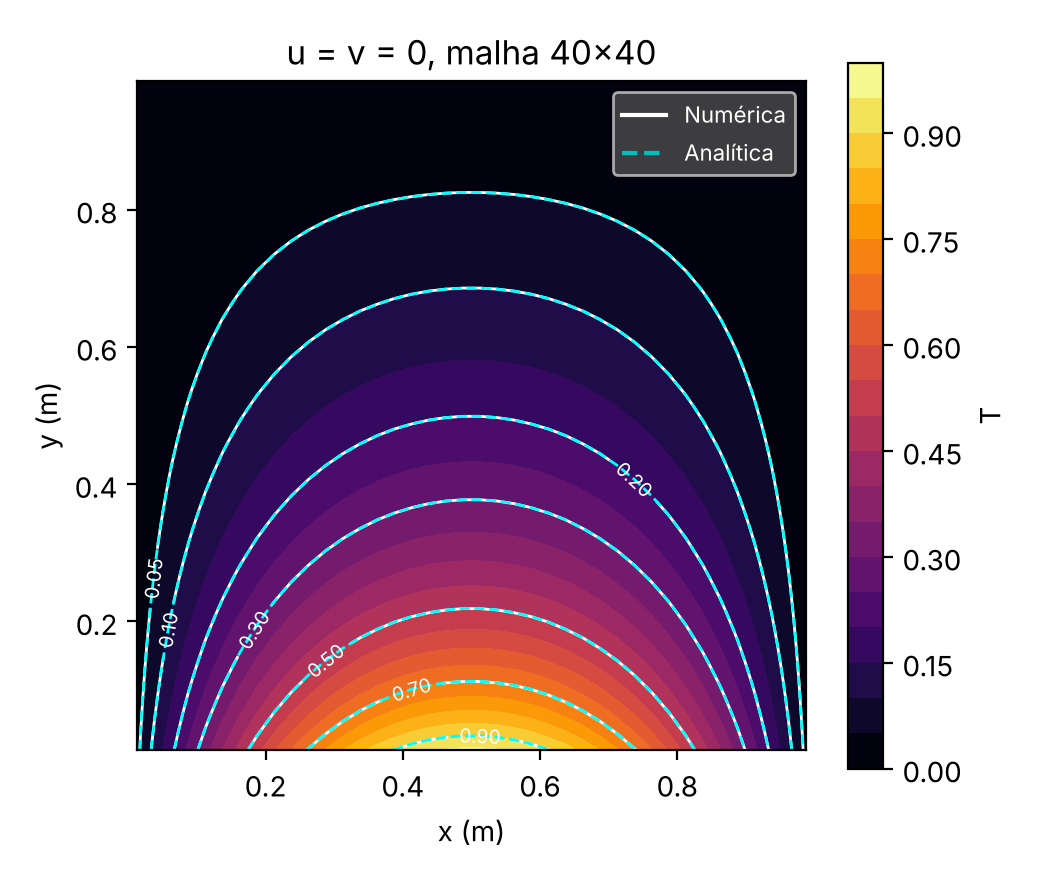
\includegraphics[width=0.62\textwidth]{L04_Q2_laplace.png}
\caption{Campo de temperatura para $u=v=0$, malha $40\times40$. Isotermas da
solução numérica (contínuas) e da analítica, Eq.~\eqref{eq:q2laplace}
(tracejadas).}
\end{figure}

\begin{table}[H]
\centering
\caption{Convergência de malha para $u=v=0$ ($a=b=1$,
$\varepsilon=10^{-10}$). Erro máximo nodal em relação à
Eq.~\eqref{eq:q2laplace}.}
\begin{tabular}{crrrr}
\hline
$N_x=N_y$ & $\Delta x$ & iterações & $|e|_{\max}$ & razão\\
\hline
10 & 0,1000 &  103 & $9{,}10\times10^{-3}$ & ---\\
20 & 0,0500 &  380 & $2{,}68\times10^{-3}$ & 3,40\\
40 & 0,0250 & 1410 & $7{,}21\times10^{-4}$ & 3,72\\
80 & 0,0125 & 5203 & $1{,}87\times10^{-4}$ & 3,86\\
\hline
\end{tabular}
\end{table}

As isotermas numéricas e analíticas são praticamente coincidentes. Com
$u=v=0$ tem-se $\alpha=0$ e $\beta=1$, e o WUDS se reduz ao CDS, de segunda
ordem: ao dobrar a malha, o erro cai por um fator que tende a $4$
($3{,}40\to3{,}86$). O número de iterações cresce aproximadamente com
$N^2$.

\vspace{0.5cm}

%======================================================================
\subsubsection*{Caso limite 2: laterais isoladas, $T=\text{cte}$ em $y=0$, $u=\text{cte}$, $v=0$}

Com as paredes laterais isoladas e $T=1$ uniforme na base, não há variação
em $x$, e o transporte advectivo em $x$ não altera o campo
($\partial T/\partial x=0$). Resta a condução unidimensional em $y$, cuja
solução é a reta
\[
  T(y)=1-\frac{y}{b}.
\]

\begin{table}[H]
\centering
\caption{Laterais isoladas, $u=\text{cte}$, $v=0$ (malha $20\times20$,
$\varepsilon=10^{-12}$).}
\begin{tabular}{crrr}
\hline
$u$ (m/s) & $\mathrm{Pe}_{\Delta x}$ & iterações & $|e|_{\max}$\\
\hline
0   & 0   & 945 & $4\times10^{-11}$\\
10  & 0,5 & 945 & $4\times10^{-11}$\\
50  & 2,5 & 945 & $4\times10^{-11}$\\
100 & 5,0 & 945 & $4\times10^{-11}$\\
\hline
\end{tabular}
\end{table}

A solução numérica reproduz a reta até o nível do critério de parada, para
qualquer velocidade. Isso confirma que o tratamento das paredes isoladas é
consistente: o fluxo advectivo que entra por uma face de cada volume é
exatamente o que sai pela outra, e a advecção em $x$ não introduz
perturbações.

\subsubsection*{Extensão: laterais isoladas, $u=0$, $v=\text{cte}$}

Um caso unidimensional mais exigente é obtido com o escoamento na direção
$y$: o problema torna-se o mesmo da Questão~1, com $T=1$ em $y=0$ e $T=0$ em
$y=b$. A solução vale para $v$ de qualquer sinal:
\begin{equation}
  T(y)=\frac{1-e^{\,\mathrm{Pe}_b\,(y/b-1)}}{1-e^{-\mathrm{Pe}_b}},
  \qquad \mathrm{Pe}_b=\frac{\rho\,v\,b}{\Gamma}.
  \label{eq:q21Dv}
\end{equation}

\begin{figure}[H]
\centering
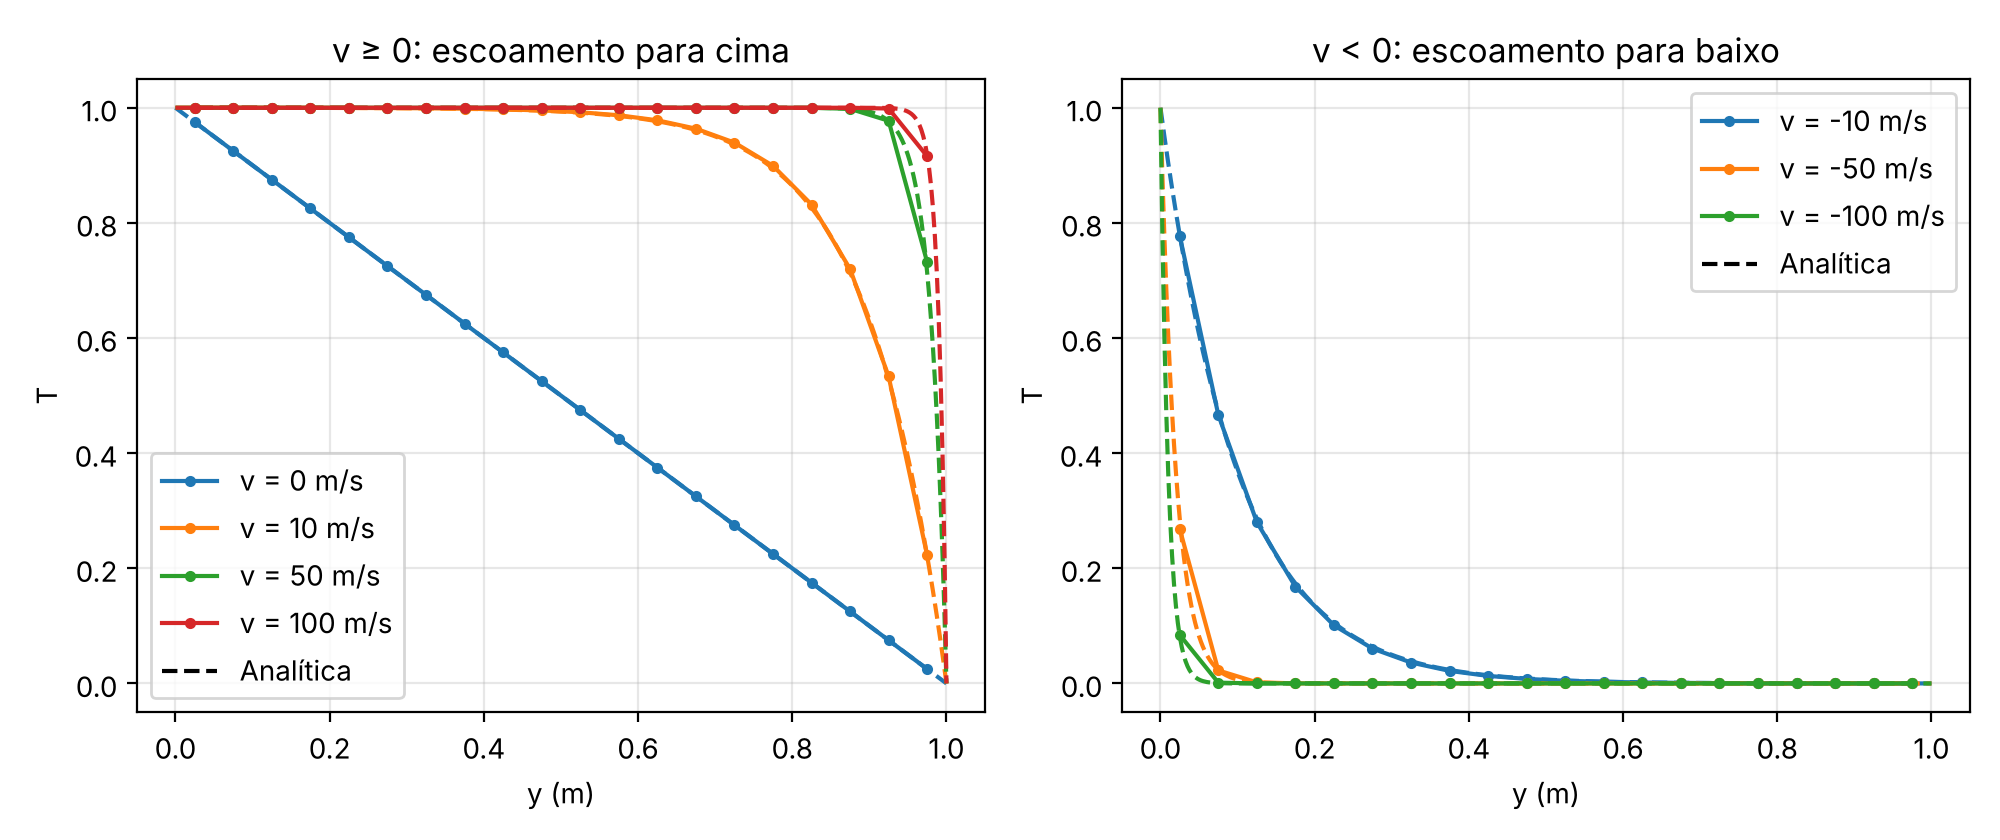
\includegraphics[width=0.98\textwidth]{L04_Q2_1D.png}
\caption{Laterais isoladas, $u=0$, malha $20\times20$: perfil vertical
numérico (pontos) e analítico, Eq.~\eqref{eq:q21Dv} (tracejado), para
escoamento para cima ($v\ge0$) e para baixo ($v<0$).}
\end{figure}

\begin{table}[H]
\centering
\caption{Laterais isoladas, $u=0$, $v=\text{cte}$ (malha $20\times20$).}
\label{tab:q2_1Dv}
\begin{tabular}{crrr}
\hline
$v$ (m/s) & $\mathrm{Pe}_{\Delta y}$ & iterações & $|e|_{\max}$\\
\hline
0    & 0    & 945 & $<10^{-10}$\\
10   & 0,5  & 297 & 0,0064\\
50   & 2,5  &  27 & 0,0181\\
100  & 5,0  &  14 & 0,0022\\
$-10$  & $-0{,}5$ & 246 & 0,0064\\
$-50$  & $-2{,}5$ &  18 & 0,0181\\
$-100$ & $-5{,}0$ &   9 & 0,0022\\
\hline
\end{tabular}
\end{table}

Os erros coincidem com os do WUDS na Questão~1 ($0{,}0064$, $0{,}0181$ e
$0{,}0022$), o que confirma que a implementação 2D recupera o caso 1D. Com
$v<0$ o escoamento entra pelo topo e sai pela base; 
os erros são exatamente os mesmos de $v>0$, pois o
problema é o espelho do anterior. A solução converge mesmo com
$|\mathrm{Pe}_{\Delta y}|=5$, e o número de iterações cai fortemente à medida
que $|v|$ cresce.

\vspace{0.5cm}

%======================================================================
\subsubsection*{Influência de $\mathrm{Pe}_{\Delta x}$ e $\mathrm{Pe}_{\Delta y}$}

Para o problema original (base senoidal, demais paredes a $T=0$), foram
combinados $\mathrm{Pe}_{\Delta x}$ e $\mathrm{Pe}_{\Delta y}$ iguais a
$0$, $1$ e $5$ em uma malha $20\times20$ com $b/a=1$, o que corresponde a
$\mathrm{Pe}_a$ e $\mathrm{Pe}_b$ iguais a $0$, $20$ e $100$.

\begin{figure}[H]
\centering
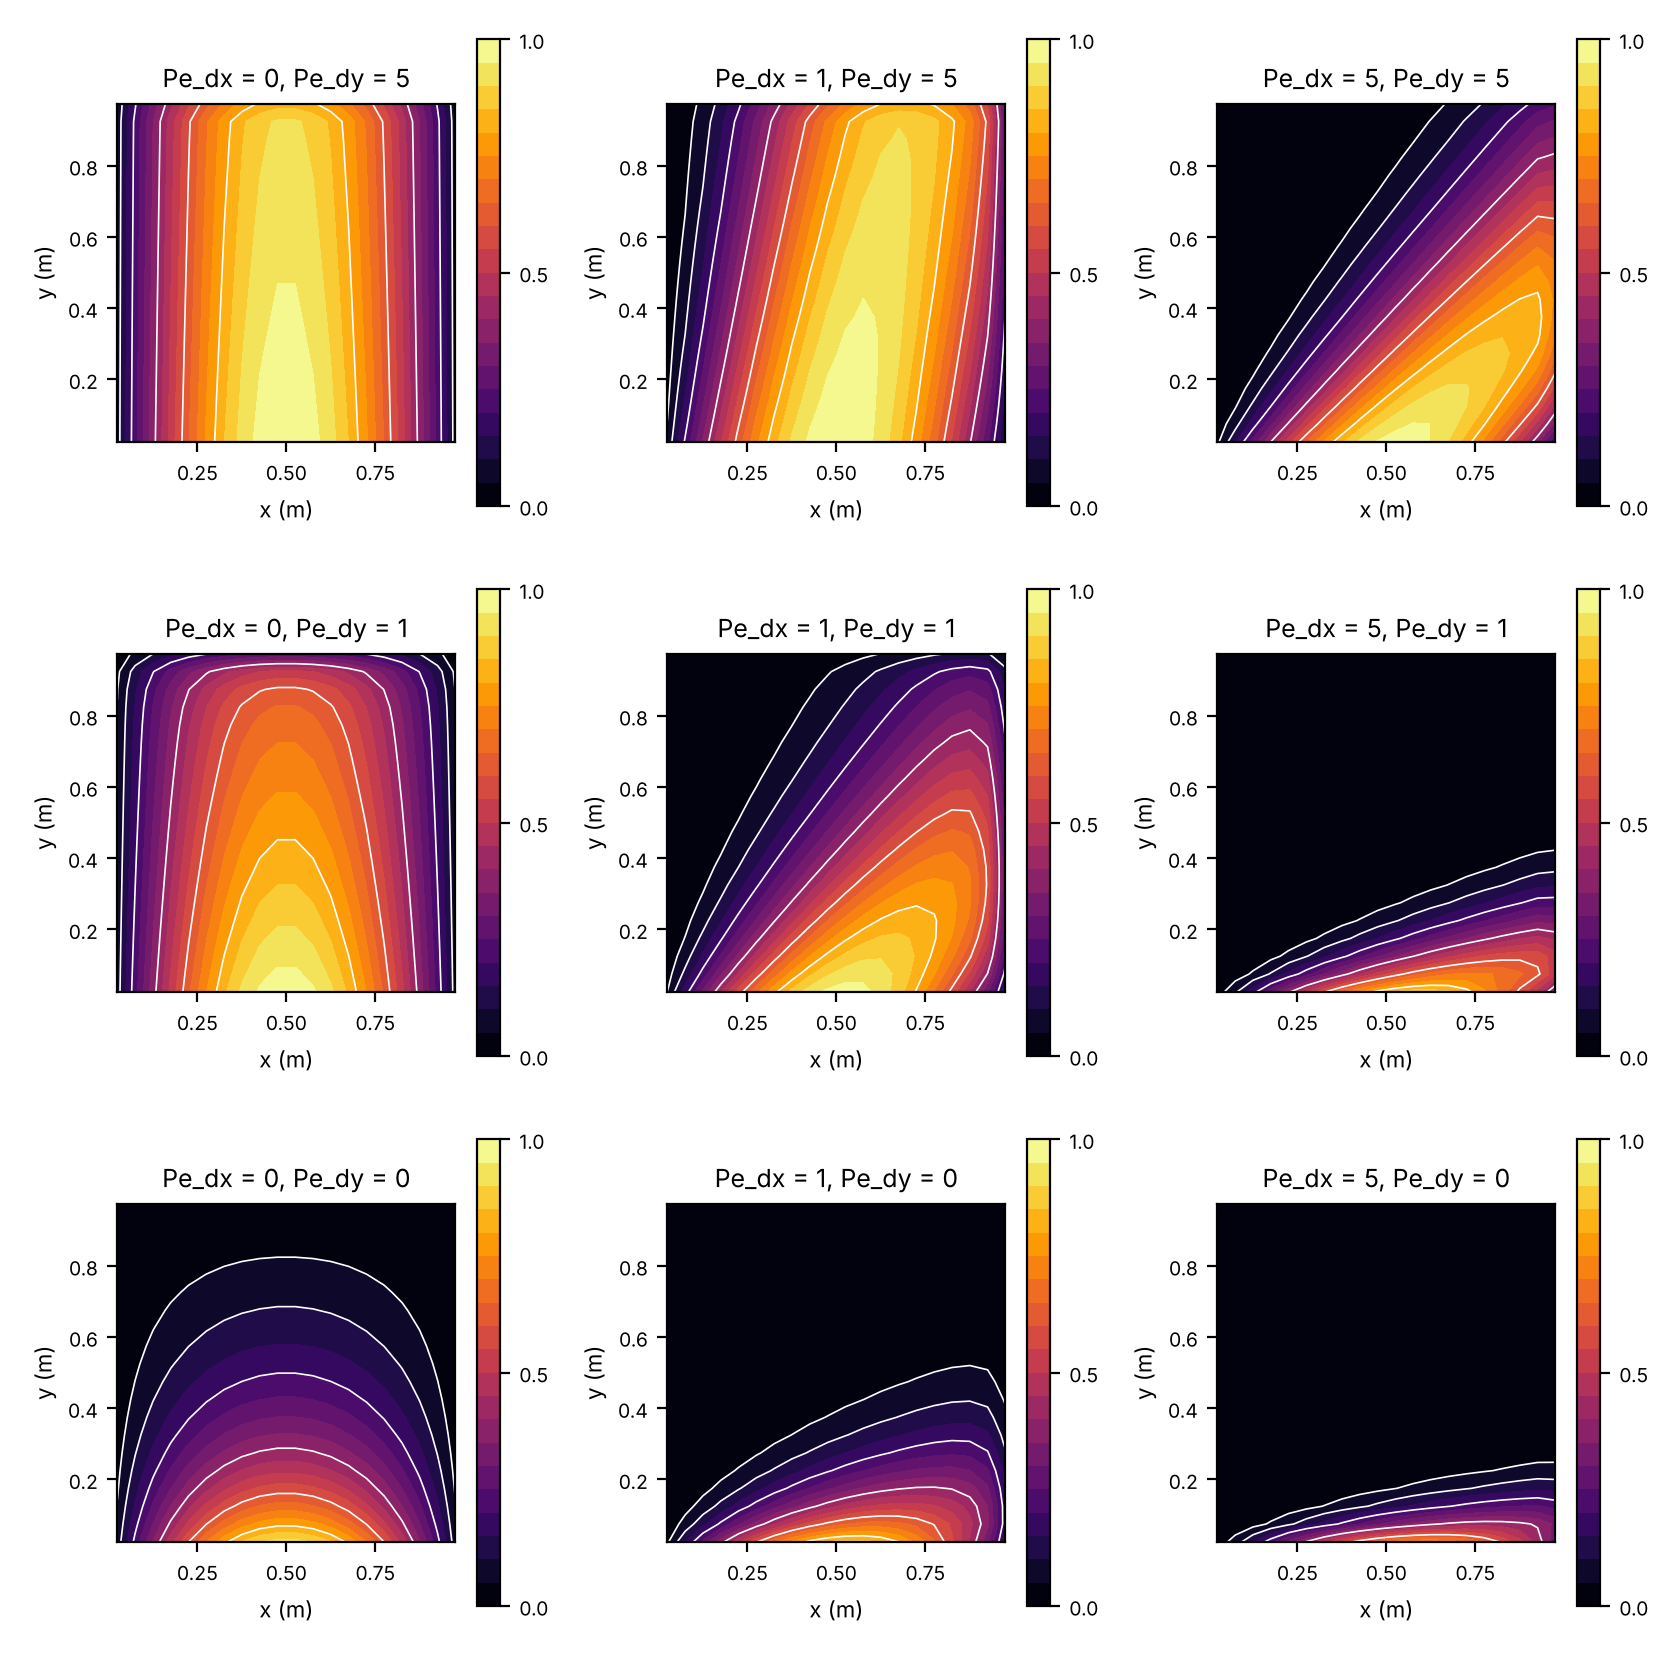
\includegraphics[width=0.92\textwidth]{L04_Q2_mapaPe.png}
\caption{Campos de temperatura para combinações de $\mathrm{Pe}_{\Delta x}$
(colunas) e $\mathrm{Pe}_{\Delta y}$ (linhas), malha $20\times20$, $b/a=1$.
Isotermas em $T=0{,}05$; $0{,}1$; $0{,}2$; $0{,}4$; $0{,}6$ e $0{,}8$.}
\end{figure}

\begin{table}[H]
\centering
\caption{Temperatura no centro da placa, $T_c=T \left(\dfrac{a}{2},\dfrac{b}{2}\right)$, e número de
iterações (malha $20\times20$).}
\begin{tabular}{c|ccc}
\hline
 & $\mathrm{Pe}_{\Delta x}=0$ & $\mathrm{Pe}_{\Delta x}=1$ & $\mathrm{Pe}_{\Delta x}=5$\\
\hline
$\mathrm{Pe}_{\Delta y}=0$ & 0,1992 (287) & 0,0186 (64) & 0,0000 (15)\\
$\mathrm{Pe}_{\Delta y}=1$ & 0,7819 (65)  & 0,3086 (43) & 0,0008 (14)\\
$\mathrm{Pe}_{\Delta y}=5$ & 0,9471 (10)  & 0,8914 (10) & 0,2296 (8)\\
\hline
\end{tabular}
\end{table}

\begin{itemize}
  \item \textbf{Advecção em $y$} ($\mathrm{Pe}_{\Delta x}=0$): o escoamento
        carrega o perfil senoidal da base para cima. Com
        $\mathrm{Pe}_{\Delta y}=5$ as isotermas ficam quase verticais e o
        seno chega praticamente inalterado ao topo; $T_c$ sobe de $0{,}20$ para
        $0{,}95$.
  \item \textbf{Advecção em $x$} ($\mathrm{Pe}_{\Delta y}=0$): o calor que
        sai da base é arrastado para leste e não tem tempo de se difundir
        para cima. A região aquecida se reduz a uma faixa junto à base,
        deslocada para a direita, e $T_c$ cai a zero.
  \item \textbf{Advecção nas duas direções}: as isotermas se alinham com a
        direção de $\mathbf{V}$. Com $\mathrm{Pe}_{\Delta x}=\mathrm{Pe}_{\Delta y}$
        a região aquecida segue uma linha inclinada a $45^\circ$; quando uma
        componente domina, a linha se inclina na direção dela.
\end{itemize}

Em todos os casos a temperatura mínima foi não negativa e o máximo não
superou o valor da base: não há oscilações, mesmo com
$\mathrm{Pe}_\Delta=5$, condição em que o CDS seria instável. O número de
iterações diminui à medida que o Péclet cresce.

\subsubsection*{Independência de malha com advecção}

Para $u=v=50$~m/s ($\mathrm{Pe}_a=\mathrm{Pe}_b=50$), a malha foi refinada de
$10\times10$ a $160\times160$.

\begin{table}[H]
\centering
\caption{Refino de malha para $u=v=50$~m/s ($\varepsilon=10^{-9}$). A
diferença é tomada em relação à malha $160\times160$.}
\begin{tabular}{crrrr}
\hline
$N$ & $\mathrm{Pe}_\Delta$ & iterações & $T_c$ & diferença\\
\hline
10  & 5,000 &   8 & 0,28967 & 0,0671\\
20  & 2,500 &  16 & 0,24850 & 0,0259\\
40  & 1,250 &  50 & 0,22733 & 0,0047\\
80  & 0,625 & 202 & 0,22273 & 0,0001\\
160 & 0,313 & 839 & 0,22261 & ---\\
\hline
\end{tabular}
\end{table}

Todas as malhas fornecem soluções limitadas e sem oscilações, mas as
grosseiras superestimam $T_c$. Com $\mathrm{Pe}_\Delta$ elevado o WUDS se
aproxima do UDS, de primeira ordem, e introduz difusão numérica. Com o
refino, $\mathrm{Pe}_\Delta$ diminui, o esquema se aproxima do CDS e a
convergência se acelera: a diferença cai de $0{,}026$ para $0{,}005$ e
depois para $0{,}0001$. A partir de $N=80$ ($\mathrm{Pe}_\Delta<1$) a
solução pode ser considerada independente da malha para fins práticos.

\vspace{0.5cm}

%======================================================================
\subsubsection*{Influência da relação $b/a$}

Foram simuladas placas com $b/a=0{,}5$; $1$ e $2$, mantendo $a=1$ e volumes
quadrados ($N_x=40$, $N_y=40\,b/a$), para $u=v=0$ e para $u=v=20$~m/s.

\begin{figure}[H]
\centering
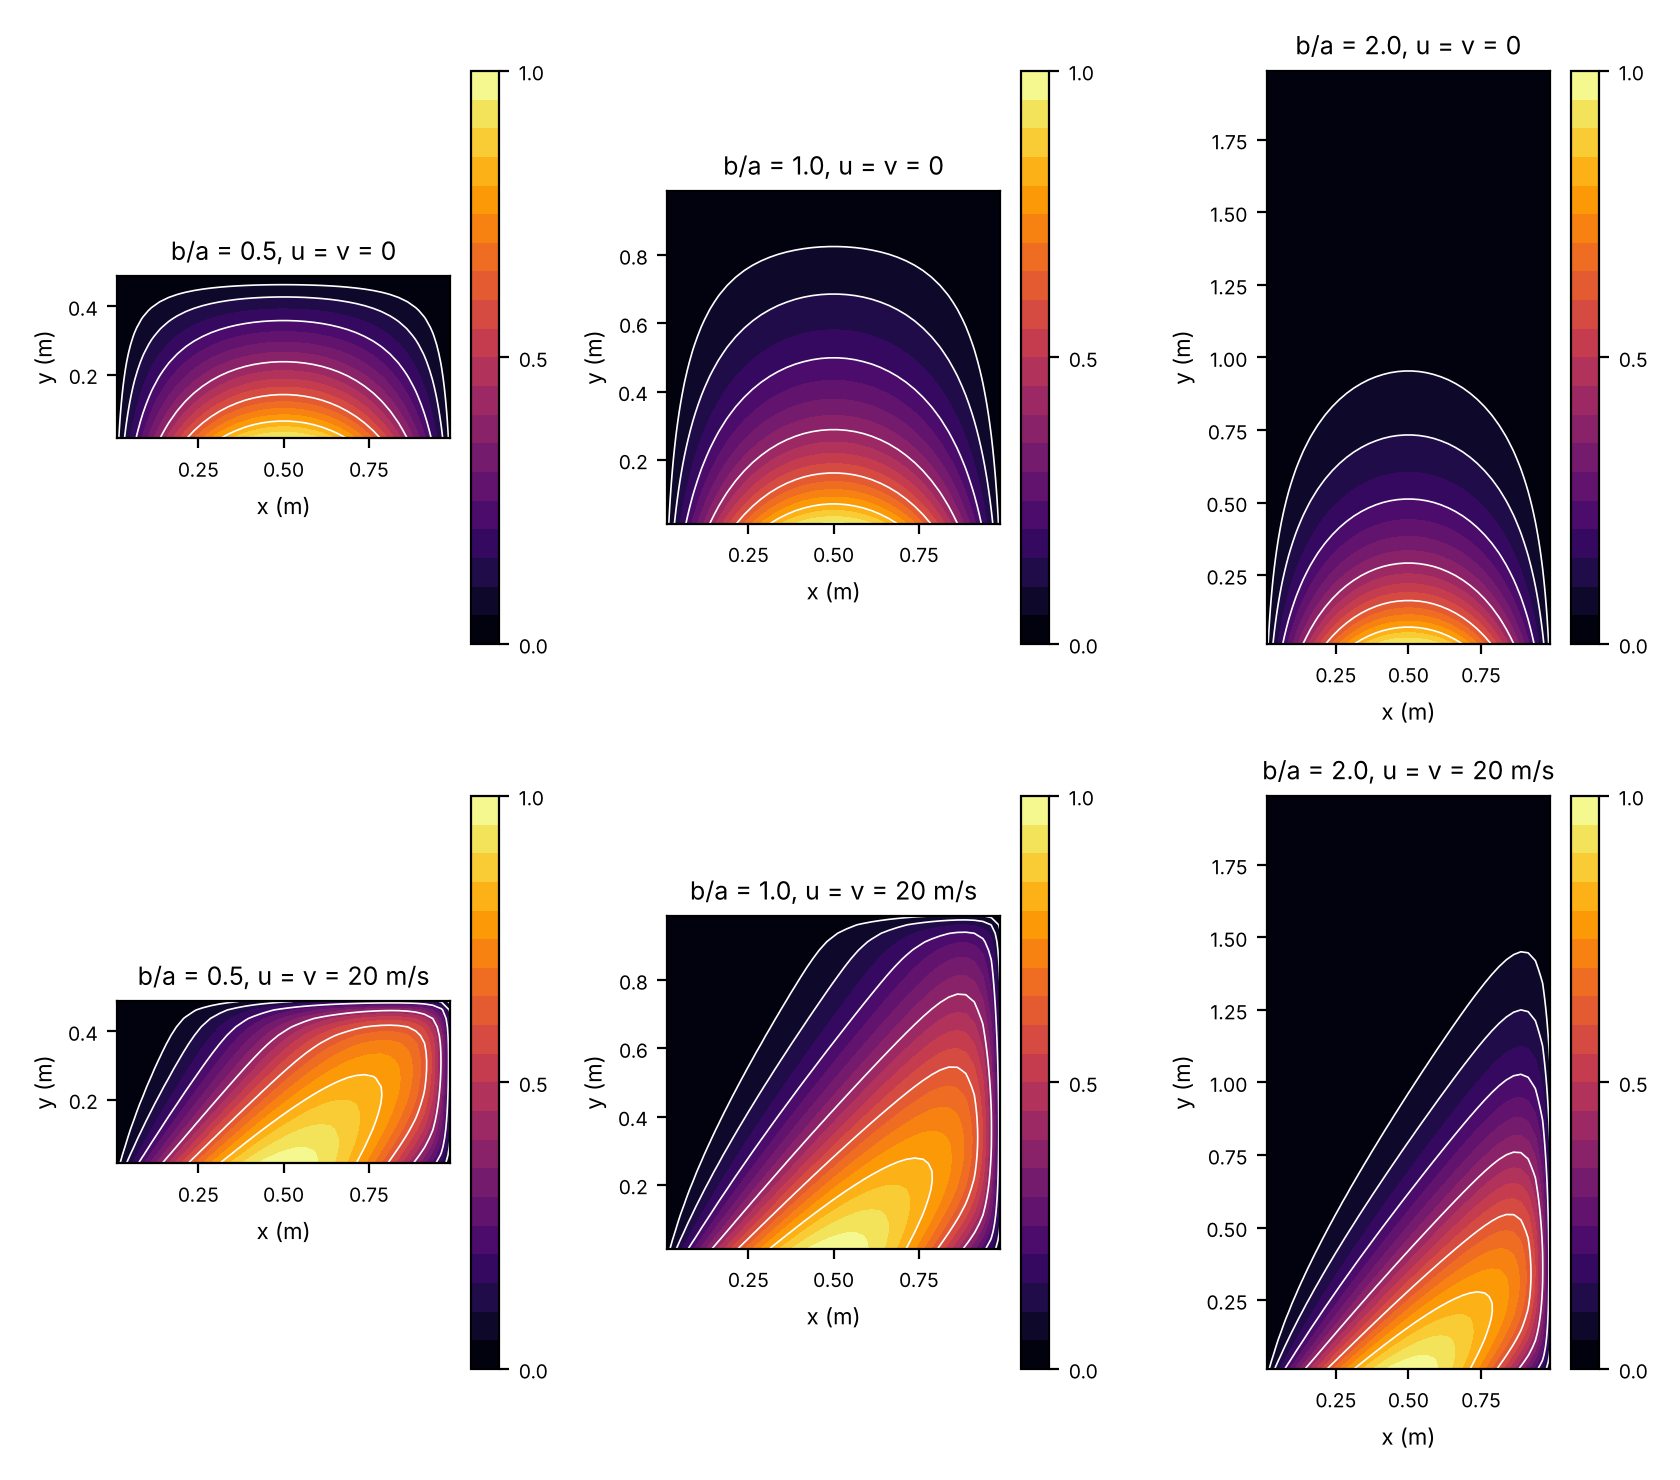
\includegraphics[width=0.92\textwidth]{L04_Q2_ba.png}
\caption{Campos de temperatura para $b/a=0{,}5$; $1$ e $2$. Linha superior:
$u=v=0$. Linha inferior: $u=v=20$~m/s.}
\end{figure}

\begin{table}[H]
\centering
\caption{Influência de $b/a$ ($N_x=40$, volumes quadrados).}
\begin{tabular}{crrrr}
\hline
$b/a$ & $|e|_{\max}$ ($u=v=0$) & $T_c$ ($u=v=0$) & $T_c$ analítico & $T_c$ ($u=v=20$)\\
\hline
0,5 & $7{,}22\times10^{-4}$ & 0,3773 & 0,3775 & 0,6500\\
1,0 & $7{,}20\times10^{-4}$ & 0,1993 & 0,1993 & 0,3065\\
2,0 & $7{,}20\times10^{-4}$ & 0,0432 & 0,0431 & 0,0429\\
\hline
\end{tabular}
\end{table}

Sem escoamento, o decaimento vertical é controlado por $\pi/a$ (largura da
placa), e não por $b$: perto da base o campo é praticamente o mesmo nas três
placas. Para $b/a=2$ o topo fica tão distante que a solução se aproxima da
de uma placa semi-infinita, $T\approx\operatorname{sen}(\pi x/a)\,e^{-\pi y/a}$;
para $b/a=0{,}5$ o topo frio comprime as isotermas. O erro em relação à
Eq.~\eqref{eq:q2laplace} é o mesmo nas três geometrias, pois depende apenas
do tamanho dos volumes.

Com escoamento, as isotermas seguem a direção de $\mathbf{V}$ ($45^\circ$
para $u=v$). Na placa baixa ($b/a=0{,}5$) ela atinge o topo e toda a placa se
aquece ($T_c=0{,}65$); na placa alta ($b/a=2$) o núcleo aquecido sai pela face
leste antes de alcançar o centro geométrico ($y=1$), que permanece frio.

\vspace{0.5cm}

%======================================================================
\subsubsection*{Velocidades negativas}

Como a base é aquecida com $\operatorname{sen}(\pi x/a)$, simétrico em relação
a $x=a/2$, o campo obtido com $-u$ tem de ser o espelho, em $x$, do campo
obtido com $+u$. Para $u=\pm50$~m/s e $v=20$~m/s (malha $20\times20$), o
desvio máximo entre os dois campos espelhados foi de $4\times10^{-16}$, com o mesmo
número de iterações (21) nos dois casos.

\begin{figure}[H]
\centering
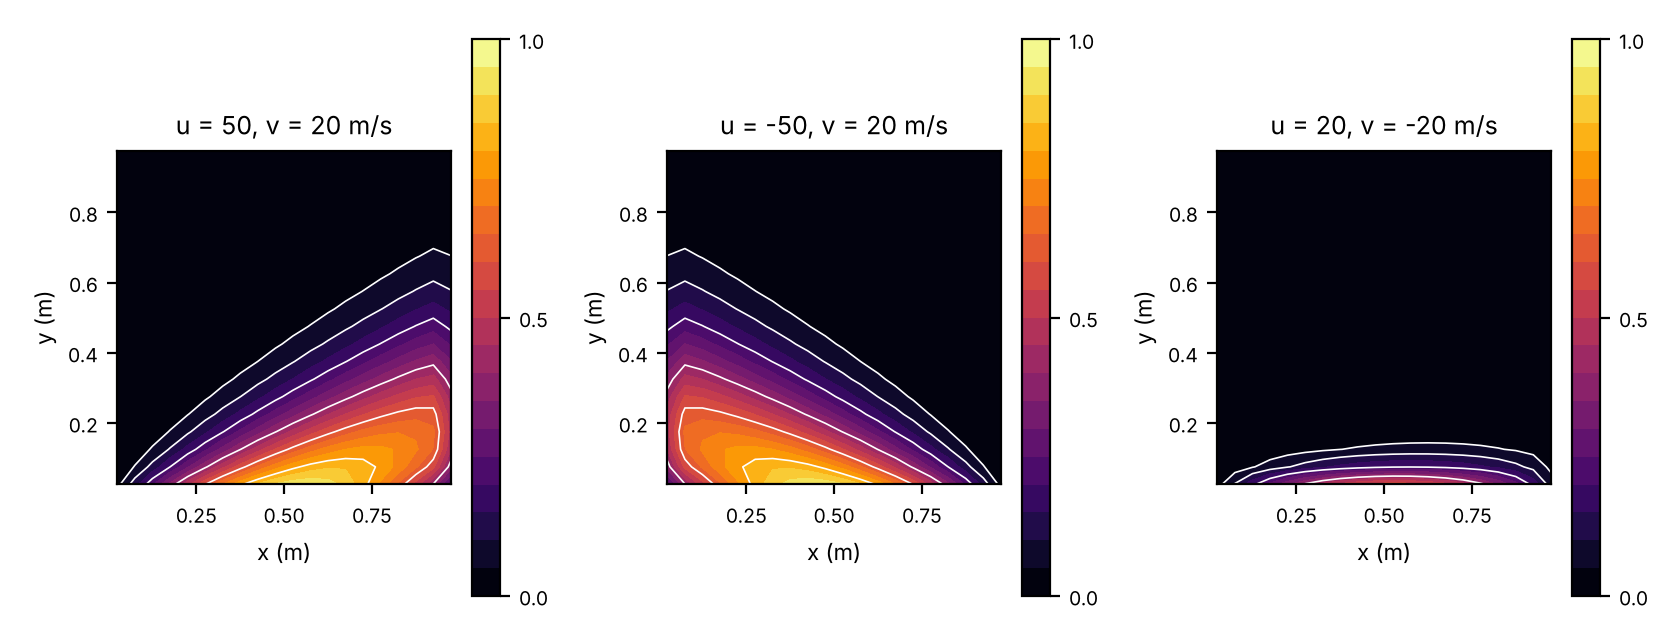
\includegraphics[width=0.95\textwidth]{L04_Q2_negativo.png}
\caption{Campos de temperatura com componentes negativas da velocidade
(malha $20\times20$).}
\end{figure}

\begin{table}[H]
\centering
\caption{Casos com velocidades negativas (malha $20\times20$).}
\begin{tabular}{rrrrr}
\hline
$u$ (m/s) & $v$ (m/s) & iterações & $T_c$ & $T_{\max}$\\
\hline
50    & 20    & 21 & 0,0249 & 0,9400\\
$-50$ & 20    & 21 & 0,0249 & 0,9400\\
20    & $-20$ & 31 & 0,0000 & 0,5855\\
\hline
\end{tabular}
\end{table}

Com $v<0$ o escoamento entra pelo topo, a $T=0$, e empurra o calor de volta
para a base: a região aquecida fica restrita a uma camada junto a $y=0$.

\vspace{0.5cm}

%======================================================================
\subsubsection*{Generalização: placa fina com troca de calor pelas faces}

Considera-se agora a placa com espessura $e$ pequena, trocando calor com o
ambiente a $T_\infty$ pelas duas faces, com coeficiente $h$. Admitindo
temperatura uniforme na espessura ($\mathrm{Bi}=he/k\ll1$), a perda nas duas
faces de um elemento $dx\,dy$ é $2h\,(T-T_\infty)\,dx\,dy$; dividida pelo
volume $e\,dx\,dy$, ela entra na equação como um sumidouro distribuído,
análogo à perda lateral de uma aleta:
\[
  S=-\frac{2h}{e}\left(T-T_\infty\right)
  \quad\Rightarrow\quad
  \frac{S}{c_p}=-m^2\,\Gamma\left(T-T_\infty\right),
  \qquad m^2=\frac{2h}{k\,e}.
\]
Na forma adimensional, a Eq.~\eqref{eq:q2adim} ganha o termo
$-M\,(T-T_\infty)$ no lado direito, com
\[
  M=m^2a^2=\frac{2\,h\,a^2}{k\,e}.
\]

Integrando no volume, o termo fonte linearizado tem $S_P=-m^2\Gamma<0$ e
$S_C=m^2\Gamma\,T_\infty$:
\[
  A_P\leftarrow A_P+m^2\Gamma\,\Delta x\,\Delta y,\qquad
  B\leftarrow B+m^2\Gamma\,\Delta x\,\Delta y\,T_\infty .
\]
Como $S_P<0$, a diagonal fica ainda mais dominante. Nada mais muda na
estrutura do programa. Adotou-se $T_\infty=0$.

\subsubsection*{Verificação}

Para $u=v=0$ a separação de variáveis continua válida, agora com
$g''-\lambda^2g=0$, $\lambda^2=(\pi/a)^2+m^2$:
\begin{equation}
  T(x,y)=\operatorname{sen}\left(\frac{\pi x}{a}\right)
  \frac{\operatorname{senh}\left[\lambda(b-y)\right]}{\operatorname{senh}(\lambda b)} .
  \label{eq:q2fonte}
\end{equation}

\begin{table}[H]
\centering
\caption{Placa com troca pelas faces, $u=v=0$ (malha $40\times40$,
$\varepsilon=10^{-10}$). Erro em relação à Eq.~\eqref{eq:q2fonte}.}
\begin{tabular}{crrrr}
\hline
$M$ & $\lambda a$ & iterações & $|e|_{\max}$ & $T_c$\\
\hline
0  & 3,142 & 1410 & $7{,}20\times10^{-4}$ & 0,1993\\
10 & 4,458 &  935 & $1{,}43\times10^{-3}$ & 0,1065\\
50 & 7,738 &  397 & $4{,}07\times10^{-3}$ & 0,0210\\
\hline
\end{tabular}
\end{table}

A solução numérica acompanha a analítica. O erro cresce com $M$ porque o
decaimento fica mais rápido (maior $\lambda$) e os gradientes junto à base,
mais intensos para a mesma malha. As iterações diminuem, pois o termo fonte
reforça a diagonal.

\subsubsection*{Resfriamento de uma chapa em movimento}

Com $M=20$ e a chapa movendo-se na direção $x$ ($v=0$), a base aquecida passa
a representar uma região de aquecimento sob a qual a chapa se desloca.

\begin{figure}[H]
\centering
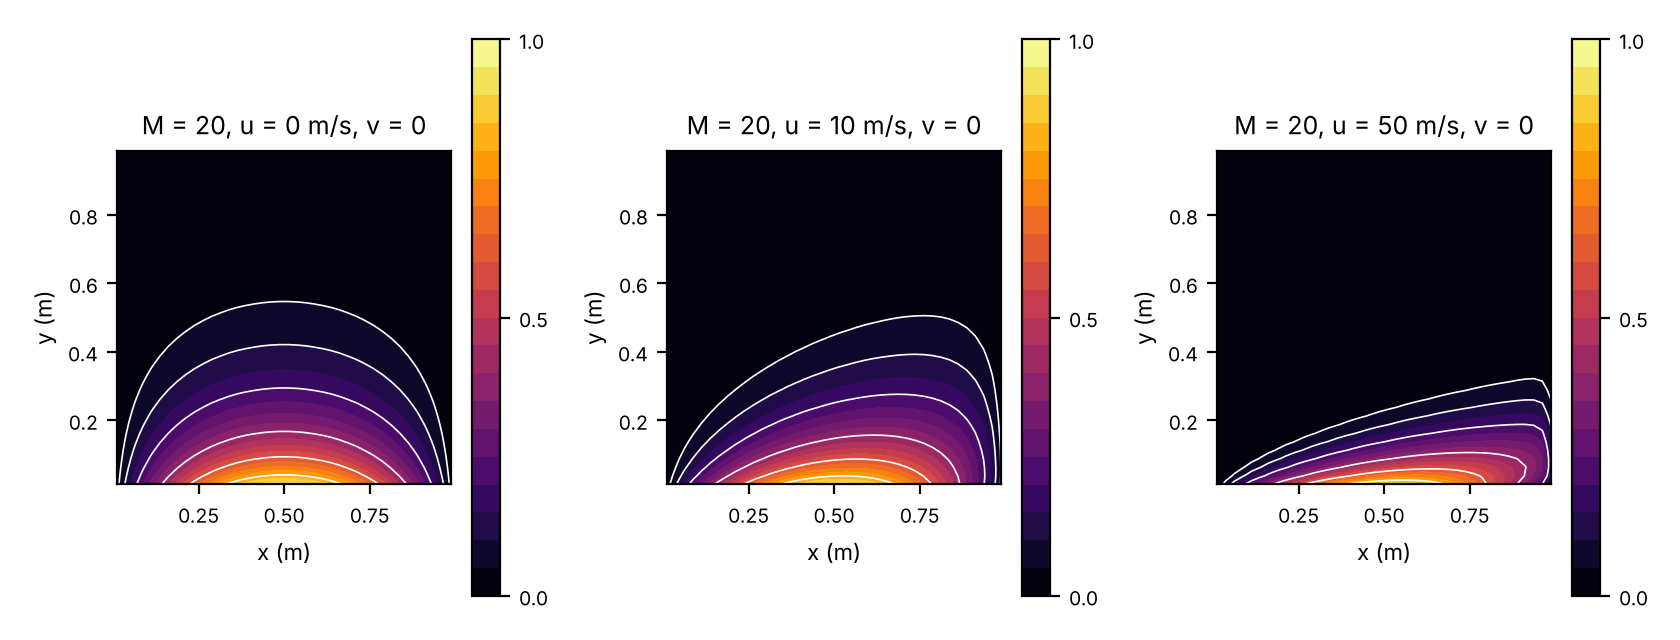
\includegraphics[width=0.95\textwidth]{L04_Q2_fonte.png}
\caption{Chapa com troca pelas faces ($M=20$), $v=0$ e $u=0$; $10$ e
$50$~m/s (malha $40\times40$).}
\end{figure}

\begin{table}[H]
\centering
\caption{Temperatura no centro da chapa para $M=20$.}
\begin{tabular}{crr}
\hline
$u$ (m/s) & iterações & $T_c$\\
\hline
0  & 698 & 0,0649\\
10 & 462 & 0,0349\\
50 &  83 & 0,0003\\
\hline
\end{tabular}
\end{table}

Comparada ao caso sem troca ($T_c=0{,}199$ para $u=v=0$), a perda pelas faces
já reduz a penetração do calor: a isoterma de $0{,}05$ desce de
$y\approx0{,}83$ para $y\approx0{,}55$. Com o movimento,
o calor é arrastado para jusante e a região aquecida se achata junto à base:
com $u=50$~m/s o centro da chapa permanece praticamente à temperatura
ambiente. Quanto mais rápida a chapa, menor o tempo de permanência sob a
fonte e menor a penetração do aquecimento.

\vspace{0.5cm}

%======================================================================
\subsubsection*{Conclusões}

\begin{itemize}
  \item O WUDS forneceu soluções limitadas e sem oscilações em toda a faixa
        estudada ($\mathrm{Pe}_\Delta$ até $5$), e reduz-se ao CDS de segunda
        ordem quando não há escoamento.
  \item A implementação foi verificada contra três soluções analíticas:
        condução pura (erro de segunda ordem), caso 1D com laterais isoladas
        (erros iguais aos da Questão~1) e placa com troca pelas faces.
  \item Com $\alpha$ com o sinal do Péclet e a interpolação WUDS entre o nó
        e o contorno em todas as faces de fronteira, a mesma formulação vale
        para qualquer sentido do escoamento, o que foi confirmado pelo teste
        de simetria. Usar diretamente o valor prescrito na face de saída
        torna o esquema instável para $\mathrm{Pe}_{\Delta}$ acima de cerca
        de $2$.
  \item O número de iterações do TDMA linha a linha cai à medida que
        $|\mathrm{Pe}_\Delta|$ cresce.
  \item A independência de malha exigiu $\mathrm{Pe}_\Delta$ da ordem de $1$ ou menor.
\end{itemize}